\documentclass[11pt]{article}

% ----- preamble (matches the other picture books in this project) -----
\usepackage[a4paper,margin=1.8cm]{geometry}
\usepackage{amsmath,amssymb}
\usepackage{array}
\usepackage{booktabs}
\usepackage{tikz}
\usepackage{tikz-cd}
\usetikzlibrary{arrows.meta,positioning,calc,fit,backgrounds,
  shapes.geometric,chains,decorations.pathreplacing,decorations.markings}
\usepackage[most]{tcolorbox}
\usepackage{parskip}
\usepackage{xcolor}

\definecolor{ink}{RGB}{40,40,40}
\definecolor{soft}{RGB}{245,245,248}
\definecolor{kas}{RGB}{30,110,190}
\definecolor{grn}{RGB}{30,140,80}
\definecolor{red2}{RGB}{200,50,50}

% the three brick colours used across this project's picture books
\definecolor{faceL}{RGB}{30,140,80}   % linearized trace  L
\definecolor{faceF}{RGB}{200,140,0}   % Frobenius / doubling  F
\definecolor{faceC}{RGB}{130,70,170}  % cyclotomic coset bookkeeping  C

\newtcolorbox{note}[1][]{colback=soft,colframe=ink,boxrule=0.4pt,
  arc=2pt,left=6pt,right=6pt,top=4pt,bottom=4pt,#1}
\newtcolorbox{leanbox}[1][]{colback=black!4,colframe=black!55,boxrule=0.4pt,
  arc=1.5pt,left=5pt,right=5pt,top=3pt,bottom=3pt,#1}
\newtcolorbox{quotebox}[1][]{colback=kas!6,colframe=kas!60,boxrule=0.5pt,
  arc=2pt,left=7pt,right=7pt,top=5pt,bottom=5pt,#1}

\tikzset{
  vtx/.style={circle,draw=ink,fill=soft,minimum size=6.5mm,font=\small,inner sep=0pt},
  fld/.style={circle,draw=faceF,fill=faceF!12,minimum size=6.5mm,font=\small,inner sep=0pt},
  obj/.style={draw=ink,rounded corners=3pt,fill=soft,inner sep=5pt,font=\small,align=center},
  brick/.style={draw=ink,rounded corners=2pt,inner sep=6pt,font=\small,align=center,
    minimum height=13mm},
  arr/.style={-{Stealth[length=2.4mm]},thick},
  dep/.style={-{Stealth[length=2.2mm]},thick,ink},
  badge/.style={circle,inner sep=0pt,minimum size=3.8mm,font=\scriptsize\bfseries,text=white},
  loopdot/.style={circle,fill=grn,minimum size=2mm,inner sep=0pt},
}
\newcommand{\bL}{\tikz[baseline=-0.6ex]\node[badge,fill=faceL]{L};}
\newcommand{\bF}{\tikz[baseline=-0.6ex]\node[badge,fill=faceF]{F};}
\newcommand{\bC}{\tikz[baseline=-0.6ex]\node[badge,fill=faceC]{C};}
\newcommand{\bX}{\tikz[baseline=-0.6ex]\node[badge,fill=kas]{$\otimes$};}

\newcommand{\tr}{\operatorname{tr}}
\newcommand{\Tr}{\operatorname{Tr}}
\newcommand{\id}{\mathrm{id}}
\newcommand{\gcdd}{\operatorname{gcd}}
\newcommand{\lc}[1]{\texttt{\small #1}}
\newcommand{\smallmat}[1]{\left(\begin{smallmatrix}#1\end{smallmatrix}\right)}
\newcommand{\ck}{\textcolor{grn}{\checkmark}}

\title{\vspace{-1.5cm}\textbf{The Trace as Memory}\\[3pt]
\large Bookkeeping of what comes back --- the patterns
\bL~\bF~\bC, the categorical loop,\\
and their relevance to Kasami / Dobbertin\\[2pt]
\normalsize \bL~linearized trace \quad \bF~Frobenius \quad \bC~cyclotomic cosets
\quad \bX~categorical trace}
\author{\small A picture book for the \texttt{Equation1} Lean\,/\,Mathlib formalisation}
\date{}

\begin{document}
\maketitle
\vspace{-1.0cm}

\begin{note}
\textbf{The thought that starts this note.} \emph{Maybe the trace is a sort of
memory --- bookkeeping, like an actual audit trail?} Yes. The trace
\emph{remembers only what returns to itself}: it discards every open path and
keeps the closed loops --- the feedback, the fixed points of $R^k$. It is
bookkeeping of self-consistency: an audit of what comes back. In this project's
case it records how each element cycles under Frobenius, summing it around its
own orbit. This booklet turns that sentence into pictures, adds
\emph{variability} (several costumes of the same idea), draws the three patterns
\bL~\bF~\bC, gives the categorical version \bX, and pins down where each one
touches Kasami / Dobbertin. Boxes marked \ck\ correspond to \lc{sorry}-free Lean
declarations in \lc{Equation1/}.
\end{note}

%======================================================================
\section*{1. Trace = memory of round trips}

Think of a walker on a graph whose adjacency matrix is $A$ (a relation drawn as
arrows). The single most useful fact is:
\[
\boxed{\ \tr(A^k)=\sum_i (A^k)_{ii}
      =\#\{\text{closed walks of length }k\}
      =\#\{x : R^k(x)=x\}\ }
\]
The power $A^k$ ``takes $k$ steps'' (composes the relation $k$ times, like
iterating a function or counting successor-shifts in a \lc{Nat}). The
\emph{trace} then throws away every walk that ends somewhere else and keeps only
the ones that land home --- the round trips. So $k$ is \emph{how many
steps/shifts}, and the trace is \emph{how many of those journeys are round
trips}.

\begin{center}
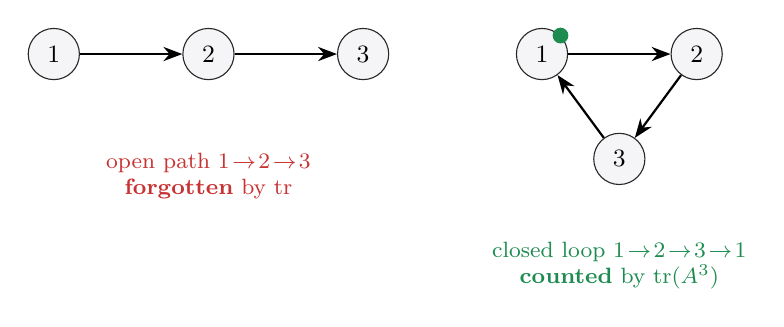
\begin{tikzpicture}[node distance=13mm]
% left: a walk that does NOT return (open path -> discarded)
\begin{scope}
  \node[vtx] (a) {$1$};
  \node[vtx,right=of a] (b) {$2$};
  \node[vtx,right=of b] (c) {$3$};
  \draw[arr] (a) -- (b);
  \draw[arr] (b) -- (c);
  \node[below=8mm of b,font=\footnotesize,text=red2,align=center]
    {open path $1\!\to\!2\!\to\!3$\\ \textbf{forgotten} by $\tr$};
\end{scope}
% right: a closed loop (round trip -> remembered)
\begin{scope}[xshift=6.2cm]
  \node[vtx] (x) {$1$};
  \node[vtx,right=of x] (y) {$2$};
  \node[vtx,below=10mm of $(x)!0.5!(y)$] (z) {$3$};
  \draw[arr] (x) -- (y);
  \draw[arr] (y) -- (z);
  \draw[arr] (z) -- (x);
  \node[loopdot] at (x.north east) {};
  \node[below=6mm of z,font=\footnotesize,text=grn,align=center]
    {closed loop $1\!\to\!2\!\to\!3\!\to\!1$\\ \textbf{counted} by $\tr(A^3)$};
\end{scope}
\end{tikzpicture}
\end{center}

\begin{note}\small
\textbf{Two readings of the same $A^k$.}
\emph{Boolean} (``does a $k$-step route exist?'') gives the composed relation
$R^k$; \emph{linear} (``how many $k$-step routes?'') counts walks. The trace only
makes sense in the \emph{linear} reading --- which is exactly why it can
\emph{count} what comes back rather than merely detect it. The fixed-point twist:
$\tr(A^k)$ picks out the $x$ with $R^k(x)=x$, i.e.\ cycles whose length
\emph{divides} $k$. That last clause is the seed of the cyclotomic-coset pattern
\bC\ below.
\end{note}

%======================================================================
\section*{2. The three patterns, drawn --- with variability}

The formalisation is built from three recurring bricks. Each is a
\emph{different costume of the same round-trip idea}; the ``variability''
columns show the same brick appearing in several guises.

\begin{center}
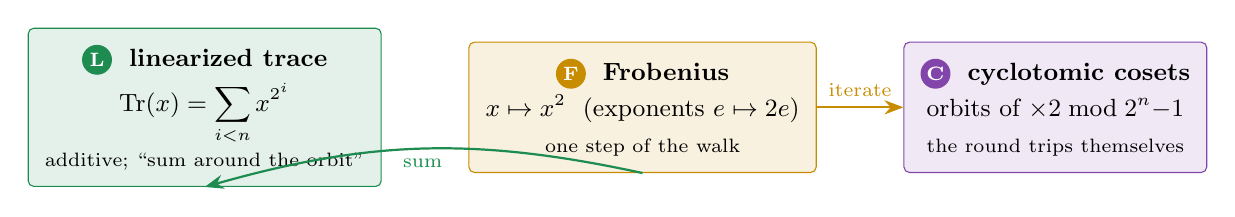
\begin{tikzpicture}[node distance=9mm]
  \node[brick,fill=faceL!12,draw=faceL] (L)
    {\bL\ \ \textbf{linearized trace}\\[2pt]
     $\Tr(x)=\displaystyle\sum_{i<n}x^{2^i}$\\[2pt]
     \scriptsize additive; ``sum around the orbit''};
  \node[brick,fill=faceF!12,draw=faceF,right=11mm of L] (F)
    {\bF\ \ \textbf{Frobenius}\\[2pt]
     $x\mapsto x^{2}$\ \ (exponents $e\mapsto 2e$)\\[2pt]
     \scriptsize one step of the walk};
  \node[brick,fill=faceC!12,draw=faceC,right=11mm of F] (C)
    {\bC\ \ \textbf{cyclotomic cosets}\\[2pt]
     orbits of $\times2 \bmod 2^n{-}1$\\[2pt]
     \scriptsize the round trips themselves};
  \draw[arr,faceF] (F) -- node[above,font=\scriptsize]{iterate} (C);
  \draw[arr,faceL] (F.south) to[bend right=14] node[below,font=\scriptsize]{sum} (L.south);
\end{tikzpicture}
\end{center}

\subsection*{2.1 \ \bF\ Frobenius --- one step of the walk}

The Frobenius map $\sigma:x\mapsto x^2$ is a \emph{bijective endorelation} on
$L=\mathbb F_{2^n}$: a permutation, so its graph is a disjoint union of cycles.
Iterating it $k$ times is $x\mapsto x^{2^k}$ --- ``$k$ shifts.'' The elements
that come back after $k$ steps, $\{x : x^{2^k}=x\}$, form the subfield
$\mathbb F_{2^{\gcdd(k,n)}}$, so
\[
\tr(\sigma^k)=\#\{x: x^{2^k}=x\}=2^{\gcdd(k,n)} .
\]
Here is the functional graph of $\sigma$ on $\mathbb F_8$ ($n=3$): two fixed
points and two $3$-cycles.

\begin{center}
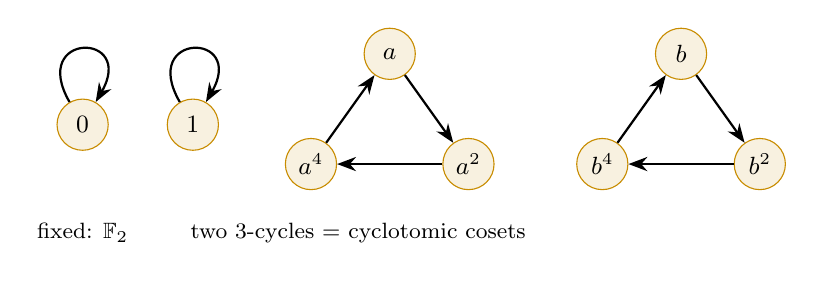
\begin{tikzpicture}
% two fixed points
\node[fld] (z) at (-3.6,0) {$0$};
\draw[arr] (z) to[out=120,in=60,looseness=8] (z);
\node[fld] (o) at (-2.2,0) {$1$};
\draw[arr] (o) to[out=120,in=60,looseness=8] (o);
\node[below=8mm of z,font=\footnotesize] {fixed: $\mathbb F_2$};
% 3-cycle A
\node[fld] (a0) at (0.3,0.9) {$a$};
\node[fld] (a1) at (1.3,-0.5) {$a^2$};
\node[fld] (a2) at (-0.7,-0.5) {$a^4$};
\draw[arr] (a0) -- (a1);
\draw[arr] (a1) -- (a2);
\draw[arr] (a2) -- (a0);
% 3-cycle B
\node[fld] (b0) at (4.0,0.9) {$b$};
\node[fld] (b1) at (5.0,-0.5) {$b^2$};
\node[fld] (b2) at (3.0,-0.5) {$b^4$};
\draw[arr] (b0) -- (b1);
\draw[arr] (b1) -- (b2);
\draw[arr] (b2) -- (b0);
\node[below=3mm of a2,xshift=6mm,font=\footnotesize]{two $3$-cycles $=$ cyclotomic cosets};
\end{tikzpicture}
\end{center}

\begin{note}\small\textbf{Variability of \bF.} Same brick, many costumes:
(i) the field automorphism $\sigma$; (ii) doubling $e\mapsto 2e$ on exponents;
(iii) the shift on cyclotomic cosets; (iv) periodicity $x^{p^r}=x^{p^{r\bmod n}}$.
In Lean: \lc{frob\_cycle}, \lc{frob\_mod}, \lc{frob\_bijective},
\lc{pow\_field\_bijective}\ \ck.
\end{note}

\subsection*{2.2 \ \bL\ Linearized trace --- summing around the orbit}

The absolute trace $\Tr(x)=\sum_{i<n}x^{2^i}$ is precisely ``walk $x$ around its
own Frobenius orbit and add up what you see.'' It is $\mathbb F_2$-linear
(additive), and it satisfies the Artin--Schreier \emph{telescope} that glues
\bL\ to \bF:
\[
\boxed{\,L_m(x)^2+L_m(x)=x^{2^m}+x\,}\qquad
\text{\scriptsize(\lc{truncTrace\_sq\_add\_self})\ \ck}
\]

\begin{center}
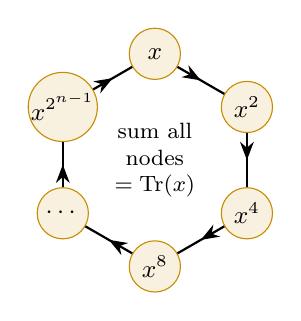
\begin{tikzpicture}[decoration={markings,mark=at position 0.5 with {\arrow{Stealth}}}]
\def\R{1.35}
\foreach \i/\lab in {0/$x$,1/$x^{2}$,2/$x^{4}$,3/$x^{8}$,4/$\cdots$,5/$x^{2^{n-1}}$}{
  \node[fld] (n\i) at ({90-\i*60}:\R) {\lab};
}
\foreach \i/\j in {0/1,1/2,2/3,3/4,4/5,5/0}{
  \draw[postaction={decorate},thick] (n\i) -- (n\j);
}
\node[align=center,font=\footnotesize] at (0,0) {sum all\\ nodes\\ $=\Tr(x)$};
\end{tikzpicture}
\end{center}

\begin{note}\small\textbf{Variability of \bL.} \lc{Tr} (full, length $n$);
\lc{truncTrace} $L_m$ (truncated, length $m$); additivity \lc{truncTrace\_add};
and --- machine-checked in \lc{Equation1/TraceLibrary.lean} --- the identification
with Mathlib's library trace: \lc{Tr\_eq\_algebraMap\_trace} shows
$\Tr = \mathrm{algebraMap}\circ\mathrm{Algebra.trace}\,(\mathbb F_2)\,L$\ \ck.
So the ``sum around the orbit'' is literally the field trace.
\end{note}

\subsection*{2.3 \ \bC\ Cyclotomic cosets --- the round trips themselves}

The cycles of \bF\ \emph{are} the cyclotomic cosets: orbits of $e\mapsto 2e$ on
$\mathbb Z/(2^n{-}1)$. A cycle of length $d$ contributes exactly when
$d \mid k$ --- this is ``fixed points of $R^k$ are cycles whose length divides
$k$.'' In the equation-(1) extract this appears in its minimal, arithmetic form:
coprimality and inverses mod $2^n-1$.

\begin{center}
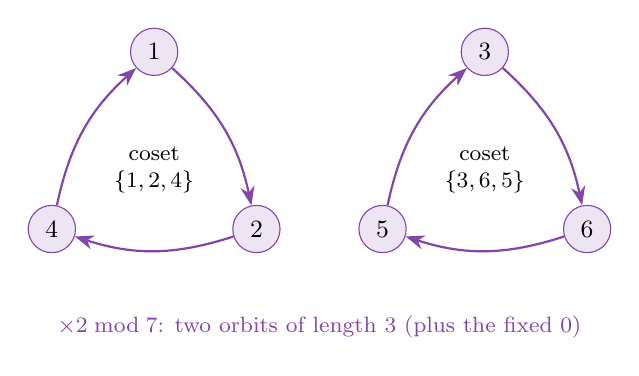
\begin{tikzpicture}
\def\R{1.5}
% coset {1,2,4} on Z/7
\foreach \i/\lab in {0/1,1/2,2/4}{
  \node[circle,draw=faceC,fill=faceC!14,minimum size=6mm,inner sep=0pt,font=\small]
    (c\i) at ({90-\i*120}:\R) {\lab};
}
\draw[arr,faceC] (c0) to[bend left=18] (c1);
\draw[arr,faceC] (c1) to[bend left=18] (c2);
\draw[arr,faceC] (c2) to[bend left=18] (c0);
\node[font=\footnotesize,align=center] at (0,0) {coset\\ $\{1,2,4\}$};
% coset {3,6,5} on Z/7
\begin{scope}[xshift=4.2cm]
\foreach \i/\lab in {0/3,1/6,2/5}{
  \node[circle,draw=faceC,fill=faceC!14,minimum size=6mm,inner sep=0pt,font=\small]
    (d\i) at ({90-\i*120}:\R) {\lab};
}
\draw[arr,faceC] (d0) to[bend left=18] (d1);
\draw[arr,faceC] (d1) to[bend left=18] (d2);
\draw[arr,faceC] (d2) to[bend left=18] (d0);
\node[font=\footnotesize,align=center] at (0,0) {coset\\ $\{3,6,5\}$};
\end{scope}
\node[font=\footnotesize,text=faceC] at (2.1,-2.0)
  {$\times 2 \bmod 7$: two orbits of length $3$ (plus the fixed $0$)};
\end{tikzpicture}
\end{center}

\begin{note}\small\textbf{Variability of \bC.} orbits of doubling; cyclotomic
cosets mod $2^n-1$; the divisibility rule ``$d\mid k$''; and the arithmetic
shadow used for Kasami: $\gcdd(2^k{-}1,2^n{-}1)=1$ with the inverse
$(2^k{-}1)^{-1}\bmod (2^n{-}1)$. In Lean: \lc{mersenne\_coprime},
\lc{inv\_mod\_exists}\ \ck. (The full difference-set / 2-rank coset theory of the
broader paper is \emph{not} in this extract.)
\end{note}

%======================================================================
\section*{3. The categorical pattern \ \bX: one loop, drawn once}

The reason all three costumes are ``the same'' is that trace is a single
categorical gadget. In a monoidal category with duals, every object $V$ has an
evaluation $\varepsilon:V^*\otimes V\to I$ and coevaluation
$\eta:I\to V\otimes V^*$. The trace of $f:V\to V$ is the one composite that
\emph{closes the wire into a loop}:
\[
\tr(f):\; I \xrightarrow{\ \eta\ } V\otimes V^*
        \xrightarrow{\ f\otimes\id\ } V\otimes V^*
        \xrightarrow{\ \mathrm{swap}\ } V^*\otimes V
        \xrightarrow{\ \varepsilon\ } I .
\]

\begin{center}
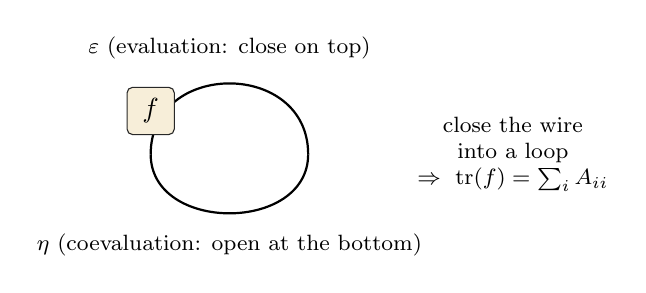
\begin{tikzpicture}[baseline]
% string diagram: a loop with a box f
\draw[thick] (0,0) .. controls (0,-1) and (2,-1) .. (2,0);   % bottom cap (coevaluation)
\draw[thick] (0,0) .. controls (0,1.2) and (2,1.2) .. (2,0); % top cap (evaluation)
\node[draw=ink,fill=faceF!15,rounded corners=2pt,minimum size=6mm] at (0,0.55) {$f$};
\node[font=\footnotesize] at (1,1.35) {$\varepsilon$ (evaluation: close on top)};
\node[font=\footnotesize] at (1,-1.15) {$\eta$ (coevaluation: open at the bottom)};
\node[font=\footnotesize,align=center] at (4.6,0)
  {close the wire\\ into a loop\\ $\Rightarrow\ \tr(f)=\sum_i A_{ii}$};
\end{tikzpicture}
\end{center}

\noindent The same picture as a \lc{tikz-cd} chain, with the $k$-th power
inserted (``take $k$ steps, then close the loop''):
\begin{center}
\begin{tikzcd}[column sep=large]
I \arrow[r,"\eta"] & V\otimes V^* \arrow[r,"R^{k}\otimes\id"] &
V\otimes V^* \arrow[r,"\mathrm{swap}"] & V^*\otimes V \arrow[r,"\varepsilon"] & I
\end{tikzcd}
\end{center}

\begin{note}\small
\textbf{Why this is exactly the memory picture.} Coevaluation \emph{opens} a
path, $R^k$ \emph{walks} it $k$ steps, and evaluation \emph{closes} it --- only
paths that can be closed survive, i.e.\ the round trips. So $\tr(R^k)$ =
feedback = fixed points of $R^k$. This is the same slogan as the
\emph{Lefschetz fixed-point theorem} (an alternating trace counts fixed points).
Basis-independence $\tr(PAP^{-1})=\tr(A)$ and $\tr(gf)=\tr(fg)$ fall out for
free, because the loop never mentions a basis.
\end{note}

\noindent \textbf{From the categorical loop to this project's trace.}
For $K\subseteq L$ and $x\in L$, multiplication $m_x(y)=x\cdot y$ is an
endomorphism of $L$, and $\Tr_{L/K}(x):=\tr(m_x)$ is the categorical loop applied
to $m_x$. Over $K=\mathbb F_2$ this unwinds (Mathlib:
\lc{FiniteField.algebraMap\_trace\_eq\_sum\_pow}) to
$\sum_{i<n}x^{2^i}$ --- the project's own \bL. So \bX\ is not a fourth pattern:
it is the hinge that makes \bL\ = ``sum around the \bF-orbit'' inevitable.

%======================================================================
\section*{4. Relevance to Kasami / Dobbertin}

\begin{center}
\renewcommand{\arraystretch}{1.3}
\begin{tabular}{@{}p{2.2cm} p{6.4cm} p{6.6cm}@{}}
\toprule
\textbf{Pattern} & \textbf{Memory / round-trip reading} &
\textbf{Role in Kasami / Dobbertin (Eqn.\ (1))} \\
\midrule
\bF\ Frobenius &
one step of the walk; $\tr(\sigma^k)=2^{\gcdd(k,n)}$ &
the squaring that generates every cycle; drives $(1)\!\Rightarrow\!(2)$ and both
cases of Thm~1 \\
\bL\ Trace &
sum around the orbit; audit of what returns &
$\Tr$ states equation (1); the telescope
$L_m(x)^2{+}L_m(x)=x^{2^m}{+}x$ is Dobbertin's ``add the $2^k$-th power to
itself'' step \\
\bC\ Cosets &
the round trips themselves; length $d\mid k$ &
$\gcdd(2^k{-}1,2^n{-}1)=1$ and the inverse mod $2^n-1$ decide when the Kasami
power $x^{2^{2k}-2^k+1}$ permutes \\
\bX\ Categorical &
the single loop behind all three &
identifies the project's $\Tr$ with the library field trace, guaranteeing the
bookkeeping is the standard one \\
\bottomrule
\end{tabular}
\end{center}

\begin{note}
\textbf{Verdict.} The memory / trace-of-powers picture \emph{does} apply to the
Dobbertin equation-(1) material: the trace \bL, the doubling \bF, and the
coprime/coset bookkeeping \bC\ are exactly the moving parts of Theorem~1, and the
categorical loop \bX\ certifies that the project's trace is the genuine field
trace (\lc{Tr\_eq\_algebraMap\_trace}, \lc{Equation1/TraceLibrary.lean})\ \ck.
Honest caveat: in this extract the ``trace of powers'' appears in its specialised
\emph{Frobenius-permutation} form ($\tr(\sigma^k)=2^{\gcdd(k,n)}$, cycles whose
length divides $k$), not as a graph-triangle count; and the broader
difference-set / 2-rank coset theory of the full paper is outside the extract.
\end{note}

%======================================================================
\section*{Appendix. The conversation this note draws on}

\begin{quotebox}\small
\textbf{Q.} Maybe trace is a sort of memory, or bookkeeping like an actual
trace?\\[3pt]
\textbf{A.} Yes --- the trace ``remembers'' only what returns to itself: it
discards all the open paths and keeps the closed loops (the feedback, the fixed
points of $R^k$). So it is bookkeeping of self-consistency --- an audit of what
comes back. In this project's case it records how each element cycles under
Frobenius, summing it around its own orbit.
\end{quotebox}

\begin{quotebox}\small
\textbf{Q.} So it is a bit like how many times a walker goes around a torus /
loop, or how in accumulator functions, or in inductive \lc{Nat} a number carries
a sense of how many steps / shifts?\\[3pt]
\textbf{A.} Exactly that flavour. $\tr(A^k)$ counts ``things that come back after
$k$ steps'' --- closed loops:
\begin{itemize}\setlength\itemsep{0pt}
\item \emph{Torus / loop:} $\tr(A^k)$ counts the ways to walk out and land home
in $k$ steps --- winding around and returning.
\item \emph{Accumulator / inductive-\lc{Nat}:} composing $R$ $k$ times ($R^k$)
\emph{is} ``take $k$ steps,'' like iterating a function or counting shifts; the
$k$ in $A^k$ is that step-count, the successor-depth of a \lc{Nat}.
\item \emph{Fixed-point twist:} $\tr$ picks the feedback --- points with
$R^k(x)=x$, cycles whose length divides $k$. For Frobenius $x\mapsto x^2$ on
$\mathbb F_{2^n}$, ``$k$ shifts'' means squaring $k$ times; the ones that return
form a subfield and the cycles are the cyclotomic cosets.
\end{itemize}
So: $k$ = how many steps / shifts, trace = how many of those journeys are round
trips.
\end{quotebox}

\vfill
\begin{center}\footnotesize
Companion to \texttt{PaperStory.tex}, \texttt{Equation1\_LEGO.tex},
\texttt{TraceMap\_Categorically.tex}, \texttt{TracePowers\_Relations.tex}.
Rebuild: \texttt{tectonic TraceAsMemory.tex}.
\end{center}

\end{document}
